\chapter{Physical model}
\label{chap:Chapter-2}
\textit{In this chapter, it's exposing the fundamental physics to understand the experimental results' trough physical model, both numerical and phenomenological. It is emphasis in symmetry properties of semiconductors, which is the base to get our model.}
\vfill
\minitoc
\newpage

\lettrine[lines=3, lraise=.1, nindent=0mm, slope=0mm]{\textbf{S}}{emiconductors} are alloy of materials with pare structural characteristics, it's the alloys which can generates an amazing quantum process that is quantum confinement.  But, all of them  couldn't possibly be achieved with understand of semiconductor bands, are bands the reason to get semiconductor heterostructures. Now, the objective is proposing the model to study Coupled Quantum Wells. The CQWs are heterostructures grown from a semiconductor substrate as GaAs as previous treated SQW (see \Cref{fig:subsection-1.2-single-quantum-well-scheme}) but coupled by a thin barrier which have a very significant role. But before to mention the objective of study this structures and the physical model which explain their experimental results  is important to call about of the symmetry and their relevance to understand the physics of these QS. \\*
Previously,  we were very repeating in the importance of semiconductor band structure, also to  in remark difficult of get them. It was saying the complexity of calculate semiconductor bands is high, by this reason it's developed models to approximate it. But, all of these couldn't be possible if it would not be taken into account the \emph{symmetry} role in physics\cite{van1989laws}. Thanks to symmetry, it's possible to understand from Quantum to Universe. It is clear that to talk the symmetry is inevitable to think in geometry or nature patterns  inherently way, but in the next sections it's established the symmetry role from the band structure calculation to  the importance in the electron behavior in CQWs structures. 

\section{The Symmetry Context}
\label{sec:chapter-2-from-symmetry}
\vspace{-10mm}
Talk about \emph{symmetry} is talk of shapes or in a romanticism way as  the natural harmony that makes something appear beautiful to us\cite{powell2010symmetry,tapp2021symmetry}. But, what is the reason the \emph{symmetry} is very important in physics?. The reason the  \emph{symmetry} is very important has to do with a \emph{transformation}, this mean that if a physical system is affected or perturbed by a thing and this appears to be exactly the same before and after that \emph{transformation}, it is said to be
\emph{invariant} under that \emph{transformation}. The symmetry of the system is made up of all the transformation operations that leave the system invariant\cite{powell2010symmetry}.

In this section doesn't have the purpose to be a one more copy or re-interpreted version of a group theory book, yes,  the group theory not symmetry theory, it's important to remember that to understand of symmetry physics of solids it's important to understand the group concept. 
In generally, a group is a set or collection of elements that obey certain criteria and are related to each other through a specific rule of interaction and obey four group axioms\cite{powell2010symmetry,cornwell1997group,muller2013symmetry}. 
It is important to remark which the heterostructure to will study is composed by GaAs/\algaas semiconductors, then  we started with the GaAs crystal to propound the symmetry role in the  CQWs.  Then, already raised the starting point,  remember that the crystal solid  can be defined as an  arrangement of atoms in strictly periodic arrays\cite{kittel2018kittel,solyom2007fundamentals}, from here arises two concepts: basis and lattice, where that last is the set of mathematical points to which the basis is attached\cite{kittel2018kittel}. These crystal concepts give place of crystal primitive cell in three dimensions also considered as the seed to reproduce a crystal. So, it gets  fundamental types of lattices defined  by a collection of \emph{symmetry} operations (rotation, translation etc.), then it's compose a lattice point group. In the three-dimensional case, the point symmetry groups require the 14 different lattices types\footnote{This lattices are known as Bravais Lattices}, where are classified into seven systems. Into these systems it's found the \emph{cubic} system, it which posses three number of lattices. Remember that the GaAs crystal is \emph{cubic},  specifically, is the type FCC lattice.  The FCC lattice is easy to imagine, if place an atom in each corner of  a cube and in a center of each face of it. Therefore, it is easier  to define  the planes and crystal directions if we take the cube faces as a reference it gets $(hkl)$ plane and the directions $\left[hkl\right]$ which must be perpendicular to a plane $(hkl)$\cite{kittel2018kittel}. 
\begin{figure}[h!]
	\centering
	\begin{subfigure}{\textwidth}
		\includegraphics[width=\linewidth]{../figures/chapter-2/symmetry/out/sym-0}
		\phantomsubcaption\label{subfig:subsubsection-2.1-crystal-rspace-a)}
		\phantomsubcaption\label{subfig:subsubsection-2.1-crystal-kspace-b)}
	\end{subfigure}
	\caption{\subref{subfig:subsubsection-2.1-crystal-rspace-a)} GaAs crystal structure in ``real space'',  this region is known as \emph{unit cell}, into that with dashed line is denoted the primitive cell. This lattice is well-defined by the vectors $\mathbf{a}$, $\mathbf{b}$ and $\mathbf{c}$, these vectors are defined as the basis vectors.  In \subref{subfig:subsubsection-2.1-crystal-kspace-b)} is schematized the GaAs crystal structure in $\boldsymbol{k}-$space, also known as \emph{reciprocal space}.}
	\label{fig:subsubsection-2.1-crystal-r-k-space}
\end{figure}

The lattice is an array of points which make the space lattice of a \cry and the repetitions or disposition of these points is controlled by ``\sym operations''\cite{chatterjee2008crystallography}. The crystal is composed by a space lattice this is a plane lattice\footnote{2D point pattern array} which have three \sym operations: \emph{Rotation axes}, \emph{Mirror plane} and \emph{Centre of Symmetry}. If add a one dimension to plane lattice it gets a space lattice, which define the unit cell of a \cry, so this adds one more \sym operation which is \emph{Rotation Inversion} or \emph{Roto-Inversion}. Then, can get \sym elements of a \cry if  apply the four \sym operations and their possible combinations. If collect that \sym elements obtains the \emph{point symmetry} or the \emph{point group of symmetry} of a \cry. 
The GaAs crystal as before mentioned is a \emph{cubic} system, but have a defined $cubic$ structure  called  as \emph{cubic zinc sulfide} or simply \emph{zincblende}. This specific \emph{cubic} structure  is characterized by arrangement of two type atoms with places  coordinates: $000$, $0\frac{1}{2}\frac{1}{2}$,  $\frac{1}{2} 0\frac{1}{2}$ , $\frac{1}{2} \frac{1}{2} 0$ for one type of these as Zn in ZnS or Ga in GaAs structure. In case of the second one atom, it has coordinates : $\frac{1}{4},\frac{1}{4},\frac{1}{4}$, $\frac{1}{4},\frac{3}{4},\frac{3}{4}$, $\frac{3}{4},\frac{1}{4}, \frac{3}{4}$, $\frac{3}{4},\frac{3}{4},\frac{1}{4}$ for S in ZnS or As in GaAs\cite{kittel2018kittel,mckelvey1966solid}.   The \Cref{subfig:subsubsection-2.1-crystal-rspace-a)} shows the unit cell of GaAs structure and into them it  dashed the primitive cell for the FCC lattice, also denoted the basis vectors  $\mathbf{a}$, $\mathbf{b}$ and $\mathbf{c}$.

In the case of symmetry of GaAs crystal, is important to remark that this symmetry can also denote in Hermann-Maguin notation  $F\overline{4}3m$ which corresponds to three fourfold rotary inversion parallel to the edges of a cube, with four threefold rotation axes parallel to the body diagonal and six mirror planes, each containing a face diagonal\cite{chatterjee2008crystallography}. The $F$ label corresponds to cubic system FCC, following by the corresponds operations.  \\*
The symmetry context before exposed can view as a macroscopic symmetry about  a crystal system, which means, is very interactive to think as a pattern well-ordered can conform a plane lattice and is intuitively work the symmetry operations. But it's not  the only  symmetry concept in crystal systems, if  we enter into crystal it found atoms or molecules which conforms it. So, the internal study of a crystal add two symmetries to the actual worked before. These ``microscopic symmetry''\cite{chatterjee2008crystallography} the make reference to $\boldsymbol{k}$-space or reciprocal space.  So, the previous concept of lattice it's also known as direct space lattice.
Thanks to X-Ray, Electron or Neutron diffraction techniques, it was possible to study the internal structure o crystal symmetries in the reciprocal space, this trough diffraction phenomena, the propagation of waves into crystal can to form well defined pattern they which are explained by the wave-vector concept\cite{malgrange2014symmetry,powell2010symmetry}. Therefore, is expected  that the electron wave function can be denoted with a lattice periodic part \bdli{u}{r} and wavelike part $e^{i\boldsymbol{k}\cdotp\boldsymbol{r}}$ so, the set of all wave vectors $\bs{k}$ corresponds to plane waves due the lattice, this is known as reciprocal lattice\cite{ashcroft1976solid}.  
Then taken into account this, and  the vectors  $\bs{a}$, $\bs{b}$ and $\bs{c}$ in reciprocal space can describe the total unit cell\cite{ashcroft1976solid,powell2010symmetry}. \\*
Finally, as a result to get the unit cell in reciprocal space and known which this is composed by lattices, these lattices are called as \emph{Brillouin} zones. Practically the \emph{Brillouin} zones are constructed by drawing the vectors $\bs{K}$ defining the reciprocal lattice and then bisecting each of these with planes perpendicular to  $\bs{K}$\cite{powell2010symmetry}\footnote{The wave vector  $\bs{K}$ is defined in\cite{powell2010chapter1} equation (1.5)}. In \Cref{subfig:subsubsection-2.1-crystal-kspace-b)} it's schematized the \brill zone to GaAs crystal structure, specifically this representation is called as \emph{ first Brillouin zone}.
To GaAs crystal it was defined the symmetry operations which compose the symmetry elements in Hermann-Maguin notation as the  point group  $F\overline{4}3m$, it's important to consider the Schoenflies notation also,  this due people often speak in terms of both, although the Hermann-Maguin notation is consider as the International notation. In Schoenflies notation, the GaAs correspond to $T_{d}$ point group. 

\subsection{The symmetry and the Band Structure}
\label{subsec:chapter-2-brillouin-bandstructure}
\vspace{-10mm}
Returning to \Cref{subfig:subsubsection-2.1-crystal-kspace-b)}, the Brillouin zone have labels which they are, importantly, this is because  each of these denote a point group symmetry. These points are:  Gamma, X, L, W, U, K.  In Schoenflies notation these correspond to: $\Gamma\to O_{h}$, $X\to C_{4v}$, $\mathrm{L}\to D_{3d}$, $\mathrm{W}\to C_{4v}$, $\mathrm{U}\to C_{2v}$, being $\Gamma$ the high symmetry point. Then, why is the importance of the \gls{BZ} role in semiconductor band structure?, the answer is the aim of this subsection. We started with the first section of this work, in it refer the importance of solution of \sch  equation, specifically at crystal structures as semiconductors. Here, the most important tool is the Bloch's theorem, it which is developed from periodic property of crystal  so, it's possible to approximate.\\*
This context is introductory and general, because this doesn't possible if  not consider the symmetry properties in crystals, in fact, \emph{the symmetry of system define the basis function to get the electron band structure}\cite{dresselhaus2007group,cardona2005fundamentals,parmenter1955symmetry,butcher2013crystalline}.  Remember that the concept of \emph{basis function} is a mathematical concept, which in quantum mechanics it's known as \emph{Wave functions}. Also, never to forget which the \emph{symmetry} concept is inherent in physics. Therefore, the Group theory establishes the game rules. 
So, the \gls{BZ} is the result of Group theory applied in crystal structures, then the \gls{BZ} is the map to understand the electron behavior in crystal structures, this defined the \ks points trough high symmetry paths, where this starts at $\Gamma$ point or $\ksm =0$.  If observe the \Cref{fig:subsubsection-1.1.1-GaAsbands-1} the horizontal axis correspond to \ks points and labeled the high-symmetry directions from $\Gamma$, then this is the \ks paths in \gls{BZ} as can see in \Cref{subfig:subsubsection-2.1-crystal-kspace-b)}. 

Previously, it's continuously mentioned which band structure calculations are difficult, so,  it will start to change the hard word to tricky, this because it's possible to make very good models and approximations taking into account the symmetry of the system. All to begins  from symmetry, the well-known models to calculate band structure starts from symmetry arguments of crystal or the semiconductor studied, through succession of  symmetry operations it knows until it's invariant, this mean doesn't change under transformation. 
Here, highlights the invariants concept, which is the connection of symmetry and Quantum Mechanics. The symmetry gets the information of the  system, while the QM the information of the state electrons. The Hamiltonian of the crystal has a symmetry which depends on their potential,  then the crystal potential posses a point group, which is invariant under any transformation. So, the solution of  the Schrödinger equation contains the state of the system. From these tools, can  propound the physics of electrons or another quasi-particle inside a semiconductor, for example in perturbation theory, starts from Hamiltonian $\mathscr{H}_{0}$ with it specific space group, but under perturbation the Hamiltonian of the system should be the sum of $\mathscr{H}=\mathscr{H}_{0}+\mathscr{H}^{\prime}$, where this last has the symmetry correspond to a subgroup of the $\mathscr{H}_{0}$ group.
This is, the principle of this work which after will be discussed with detail. While the solution of Schrödinger equation with the total Hamiltonian $\mathscr{H}$ will result in the energy spectrum $E(\boldl{k})$ along of the \gls{BZ}. Being a crystal system and the potential is the periodic, it's to hope which a multiband spectrum. Although here doesn't consider the degeneracy\footnote{This is due to the  linear independent solutions, which corresponds to one energy, this mean $m-$fold  band degeneracy at the point $\boldl{k}$\cite{bir1974symmetry}} term, it's evident which the Group Theory has the solution, in general words,   are the irreducible representations of the symmetry group which determine the dimension of degeneracy\cite{bir1974symmetry}. \\*
\emph{Thus the band structure as a whole exhibits the symmetry characterized by the crystal}\cite{bir1974symmetry}.
\\
All previous it's about of an ideal crystal, then it's possible to get exact solutions of Schrödinger equation. But, to determine in detail the spectrum $E(\boldl{k})$ throughout the \gls{BZ}, one needs a numerical solution of the Schrödinger equation. In previous sections, it shows the results of apply \gls{TB} method to GaAs bulk, this method parts from Bond Orbital Model\cite{harrison1973bond,vogl1983asemiempirical,slater1954simplified}, in this case, the basis functions it's forming linear combinations of atomic orbitals (LCAO) to specific symmetry group\cite{dresselhaus2007group}. \\*
In this method, the importance is the arrangement of atoms and their orbitals considered, for \Cref{fig:subsubsection-1.1.1-bulk-1} these are $sp^{3}$. 
In another way, in the case of \gls{kp} method, apart from perturbed model, but in both the main idea it's found the \ks-points correspond to the symmetry of the system. In another way, in the case of \gls{kp} method, apart from disturbance model, but in both the main idea it's found the \ks-points correspond to the symmetry of the system. The difference apart from their basis is the efficiency in their applied over semiconductor structures, this means that the \gls{kp}-method is appropriate in a small region of \gls{BZ} to describe $E{(\boldl{k} )}$, therefor is the preferred option to describe semiconductor bands around of $\Gamma$, while if the idea is describing $E{(\boldl{k})}$ in an extended region of the \gls{BZ} the \gls{TB}-method is the correct\cite{dresselhaus2007group,bir1974symmetry}. In any way, the symmetry establishes the basis to get semiconductor band structure, no matter the method this, includes the first principle methods as DFT, which requires the symmetry information of the system to get the pseudopotentials and the geometric optimization to enhance calculations.

Although the symmetry concept is the base, the principal objective in this work you have to see the consequences of symmetry under in a non-direct perturbation, this mean, if it has GaAs bulk-semiconductor this has one defined point group $T_{d}$. When applied it a perturbation, as an electromagnetic perturbation the principal symmetry group it's reducing to a subgroup of itself. This is to mean which the subgroup is also invariant. This conception is also knew or called \emph{symmetry breaking}. It this concept, it was employed at first time by Pierre Curie at ended of nineteenth century\cite{curie1894symetrie,sep-symmetry-breaking}, It this concept, it was employed at first time by Pierre Curie at ended of nineteenth century, he establishes that, if happens thing which doesn't allow system invariance, so the original symmetry it's lowered then,  this mean which symmetry is broken. 
But, what is  the importance to focussing on that?. The importance of symmetry breaking is the physical effects that are presents, the properties of semiconductors changes under reduce symmetry and this can observe in band structure.  In the next section will be discussed the importance of ssymmetry breaking in semiconductors and above all over QWs. 



\section{Symmetry breaking in CQWs}
\label{subsec:chapter-2-symmetry-breaking}
\vspace{-10mm}
\begin{figure}[H]
	\centering
		\includegraphics[width=\linewidth]{../figures/chapter-2/symmetry/out/sym-1-wob}
	\caption{In this figure, it's schematized the atom arrangement of \algaas/GaAs/\algaas single QW. At bottom can see the atom structure assuming the Al concentration to barriers, then, in middle of figure draws the conduction band edge as a potential profile, at interfaces between the change from barrier to well and vice versa,  are located the matched atoms, here it can observe that at these positions (interface) the symmetry of changed.  At top, it's added the atoms' basis where it has taken the Arsenic as central atom, and scheme the continues rotation over the $y$-axis. }
	\label{fig:subsubsection-2.2-qws-symmetry}
\end{figure}
The symmetry breaking, it's the basis for the physical model in this work. Starting from the general and brief concept of the symmetry importance in the Solid State viewed in the past section will arise the symmetry role and the reduced symmetry in CQWs. Before starting the history, it's important to clarify that the SOC isn't considered in this work, although in the future works of the \gls{lflm} are considered, and they study spin phenomena in CQWs. Then, to start in terms of symmetry the GaAs bulk has $T_{d}$ point group, without intention to minimize the operations only focussing on their subgroups this due as before mentioned if the symmetry is lowered then the point group reduces to one of subgroup\cite{dresselhaus2007group}. So, in the superlattice case the symmetry reduces at interfaces due to the change of atom species, that is to say, if it parts from GaAs and added an AlAs or \algaas lattice the new atom structure reduce symmetry elements that can be done then the point group $T_{d}$ it's reduce. 
Let's discuss first the simple QW GaAs/\algaas structure grown over $\left[001\right]$ direction, if suppose that the \algaas/GaAs and GaAs/\algaas interfaces\footnote{Another nomenclature usually used is A/B interfaces, being reference to two dissimilar atoms.} are ``perfect'', this mean the QWs structurally are perfect,  the symmetry of system it's reduced to from $T_{d}\to D_{2d}$ \cite{magri2000anticrossing,ivchenko1996heavylight}.  \\*
If taken into account a common atom as in this case the As atom as can see in 
\Cref{fig:subsubsection-2.2-qws-symmetry} and consider that structures growth (001)-oriented lack of translational symmetry\cite{ivchenko1996heavylight}, then in a single QW, the translational invariance along $z$ axis is lost\cite{tronc2000bound} as can see in \Cref{subsec:chapter-2-symmetry-breaking}. Is so fact which the visualization of symmetry operations ins't trivial, it can support each other with  open software library as \gls{Spglib} or \gls{ase}  symmetry functions, these are great tool which has an iterative alghoritm under applied recursive operations. If set the arrangement of atoms as the bottom of \Cref{fig:subsubsection-2.2-qws-symmetry}, sorting the atoms positions as As-Al-Ga-Ga-As-Al super lattice then at the center of heterostructure the GaAs atoms to finally complement with the heterostructure composed by the first super lattice. Then, it's applies over these the continuous operations under \gls{ase} package the result is the $P\overline{4}m2$ symmetry in terms of international notation, therefore the $D_{2d}$ point symmetry group. 
Although that is well-known and described at \cite{tronc2000bound,ivchenko1996heavylight,glazov2018electron,krebs1996giant,magri2000anticrossing,chen2002interface,ivchenko2008spinphoto}, the use of package software will be got a powerful tool to developed future works. So, in order to understand reducing symmetry from $T_{d}\to D_{2D}$ of QW grown on the (001), the $z_{_{\parallel}}(001)$ direction becomes inequivalent to both $x_{_{\parallel}}(100)$ and $y_{_{\parallel}}(010)$ directions, hence the symmetry is reducing. 

In therms of band structure the symmetry breaking, or symmetry reducing, generate changes, above all over the VB of QWs. This was expected, the reason is the due to the \gls{BZ} zone is reduce to $\Gamma$ point. From here starts the relevance of $\Gamma$ and the events which ocurrs are the next: the first one event which occurs is over VB, due to the \gls{BZ} is reduces to  $\Gamma$ the \gls{VB} it splits for heavy- and light-holes. This is, from bulk as show the band structure in \Cref{fig:subsubsection-1.1.1-GaAsbands-1} the \gls{VB} is four-fould degenerate, then in QWs the heavy- and light- holes bands splits, so,  it gets two-fold degeneracy as shows in \Cref{fig:subsection-1.2-single-quantum-well-scheme2}. In fact, when refer to $\Gamma$ in really it's refer to near band extrema, in case of GaAs and \algaas  being direct band gap semiconductors this really clearly. The consequences of bands split it's the reazon which the effective mass approximation (\gls{efa}) can works, thanks to that the  \sch's equation can solve as one dimensional equation over both \gls{CB} and \gls{VB} band  under structure material parameters. 
Then, the facility of solve \sch's equation it's limited to only getting information about transitions, it is important to remember which this solution is over real-space, for this reason, it says that the potential profile is called a band edge profile and can't confuse with the band structure. So, this is the principle of symmetry reduction in QWs structures, in the next section will be addressed the symmetry in CQWs structures and the mechanisms to reduce it. 


	


\subsection{Coupled Quantum Wells}
\label{subsubsec:chapter-2-coupled-quantum-wells}
\vspace{-10mm}
The symmetry breaking doesn't only wight in mathematical aspect, for physics this concept with leads to discover many important and exotic phenomena. When a system reduces its symmetry, their physical properties changes. It's the change in physical properties which reason to study it, in semiconductors as QWs the symmetry breaking starts with modify their band structure (fingerprint) splitting the valence band and reducing the degeneracy, although it  can be the first one to appear  their consequences get more relevance. \\*
In therms to study changes in physical properties in this work it's focus on optical properties, the light matter interaction gets information about the symmetry breaking through transitions.  The GaAs QWs as a direct band gap semiconductor are excellent platform to study light-matter interaction and the effects on symmetry. It's important to remark  that from here the excitons  played it  an important role, in fact, over them falls  the physical interpretation of optical properties.  

\begin{figure}[h!]
	\centering
	\begin{subfigure}{\textwidth}
		\includegraphics[width=\linewidth]{../figures/chapter-2/symmetry/out/sym-2-wob}
		\phantomsubcaption\label{subfig:subsubsec:chapter-2-scoupled-quantum-wells-a}
		\phantomsubcaption\label{subfig:subsubsec:chapter-2-scoupled-quantum-wells-b}
	\end{subfigure}
	\caption
	{
		General scheme to describe a SCQWs structure. In this case, the barriers are it composed by \algaas and the wells are of GaAs with the same width ($d_{1}=d_{2}$), while the coupling barrier also composed by \algaas. In top \subref{subfig:subsubsec:chapter-2-scoupled-quantum-wells-a} denotes both  CB and VB  edges profiles over $z$-axis (Real-space) direction. Then in bottom \subref{subfig:subsubsec:chapter-2-scoupled-quantum-wells-b}, it represents the atoms structure to CQWs. 
	}\label{fig:subsubsec:chapter-2-scoupled-quantum-wells}
\end{figure}

Then, in the case, of Coupled Quantum Wells (\gls{CQWs}) through excitons get optical properties really it's interesting, although, to get that properties the CQWs should get a double reduce symmetry from $T_{d}$ , even if that's not obtained it's important to anisotropy spectroscopy get it as a basis. 
Then, firstly, it's start with the symmetric coupled quantum wells (\gls{SCQWs}), these are QWs with same width and coupled with a thin barrier, this barrier must be enough thinner so that electron wave function can be overlapping along potential of the two wells. 
For these structures the symmetry is also $D_{2d}$ as in single QW, it's important to say which, if they aren't  consider the  interface defects as roughness it's possible to consider  ideal interfaces, then the same symmetry operations works in both single QW like a SCQWs. 

From \Cref{fig:subsubsec:chapter-2-coupled-quantum-wells} it's possible to compare which in contrast with the SQW (\Cref{fig:subsection-1.2-single-quantum-well-scheme}) is the same case with exception to the two QWs, although it's true that the technology of growth it's really accurate, the interfaces aren't be exempt  free of them. Even, the rough by possible of Al impurity can cause the possible segregation of this, then it's important the Al concentration $x$ \cite{chand1990origin,tillmann2002direct}. Even tought, an interface growm over (001) is $C_{2v}$, if consider structurally perfect as \gls{SQW} or \gls{SCQWs}, the overall symmetry of both interfaces is $D_{2d}$\cite{magri2000anticrossing}.

\begin{figure}[h!]
	\centering
	\begin{subfigure}{\textwidth}
	\includegraphics[width=\linewidth]{../figures/chapter-2/symmetry/out/sym-3-wob}
	\phantomsubcaption\label{subfig:subsubsec:chapter-2-acoupled-quantum-wells-a}
	\phantomsubcaption\label{subfig:subsubsec:chapter-2-acoupled-quantum-wells-b}
	\end{subfigure}
	\caption
	{General scheme corresponds to ACQWs structure.
	As in \Cref{subfig:subsubsec:chapter-2-scoupled-quantum-wells-b}, the structure is basically same both in barriers composition and dimensions as well as the coupling barrier, only changes the relative position of this. Then, result that one of QW is wider than other ($d_{1}<d_{2}$), so, this reason causes the asymmetry in structure. Also, here in top 
	\subref{subfig:subsubsec:chapter-2-acoupled-quantum-wells-a} draws the potential profile along $z$, and bottom 
	\subref{subfig:subsubsec:chapter-2-acoupled-quantum-wells-b} scheme the atoms structure where is clear that only changes coupling barrier relative position with respect to \Cref{subfig:subsubsec:chapter-2-scoupled-quantum-wells-b}
	}\label{fig:subsubsec:chapter-2-acoupled-quantum-wells}
\end{figure}

Remember that as Courie mentioned\cite{curie1894symetrie,sep-symmetry-breaking,shubnikov1988works}:  a system under perturbation reduces their symmetry to a subgroup of  original symmetry group, then, if now starts with $D_{2}$ symmetry this subgroup can only reduce to a subgroup of six possibles, into them is $C_{2v}$ subgroup. Previously it mentioned which, exist several mechanisms can reduce the symmetry, these are usually called  perturbations. These perturbations can be nature by different sources, \emph{in this work  has been it found a novel source which reduces the symmetry,  in other words,  broken symmetry  without needed external source as applied electric or magnetic fields}.  \\*
In the next section, it details the reason which it's called  a novel source of reduce symmetry, therefore, before continue it's important to mentioned that the simple reason of modify the one well width in CQWs structures makes the system loses fourfold rotations over $z_{_{\parallel}}(001)$  then, the symmetry it reduces. 

If compares \Cref{fig:subsubsec:chapter-2-scoupled-quantum-wells,fig:subsubsec:chapter-2-acoupled-quantum-wells} it's clearly that the representative part of the coupling barrier only shift over $z$, this allows to simulate a \gls{ACQWs} heterostructure, this mean which QW is wider than the other, so, it gets an asymmetric structure which along $z$ losses the rotation symmetry. Also, if it's uses symmetry code packages as \gls{ase} or \gls{Spglib} which applies consecutively symmetry operations to both CQWs structures, it results in a $D_{2d}$ and $C_{2v}$ for \gls{SCQWs} and \gls{ACQWs} respectively.  
 
\subsection{Special symmetry reduction from $D_{2d}\to C_{2v}$}
\label{subsubsec:chapter-2-special-symmetry}
\vspace{-10mm} 
The importance of $C_{2v}$ point group around of QWs system is attractively to study properties of them, over all quantum properties as ``spin'' \cite{andrada1997spin,luo2015supercoupling,ivchenko2008spinphoto,glazov2018electron,winkler2003spin,ohrmann2004anomalousspin}. Also, it's very important the quantum mixing which exhibits as a result of symmetry breaking, in fact, latter in \Cref{subsec:chapter-3-ras} it presents the result of RAS experiments,  which are the result of hole mixing. The anisotropy experimental measured it's caused due to the mixing at \gls{VB}, therefore it's a direct cause of symmetry. \Cref{fig:subsubsec:chapter-2-special-symmetry--roadmap} shows and schematics the roadmap to get a QWs structures with $C_{2v}$ symmetry. This starts at the left with asymmetrical structures\Cref{subfig:subsection-1.2-single-quantum-well-scheme2-a)}, this asymmetry is related with the potential, exists a variety of them but the objective it's practically the same, the asymmetric potential profile it can be obtained by: asymmetric barrier, this can be due to the change of semiconductor type between adjacent barriers, i.e.,  AlAs/GaAs/\algaas structure, this can interpret as high barrier/well/low barrier\cite{koopmans1998microscopic}.Another way of them,  is caused of a barrier  it's under gradient composition\cite{english2013effect,eldridge2011spinorbit}. The end case under asymmetric potential consideration shows in \Cref{subfig:subsubsec:chapter-2-roadmap-c}, this case is due in one of the barriers is intentionally ``inserted'' an atom from other specie\cite{yu2015tuning}, this causes an asymmetric potential profile. Finally, it display the our CQWs structure, in comparison with all above firstly it has two wells, therefore reduced symmetry it be 

\begin{figure}
	\centering
	\begin{subfigure}{\textwidth}
		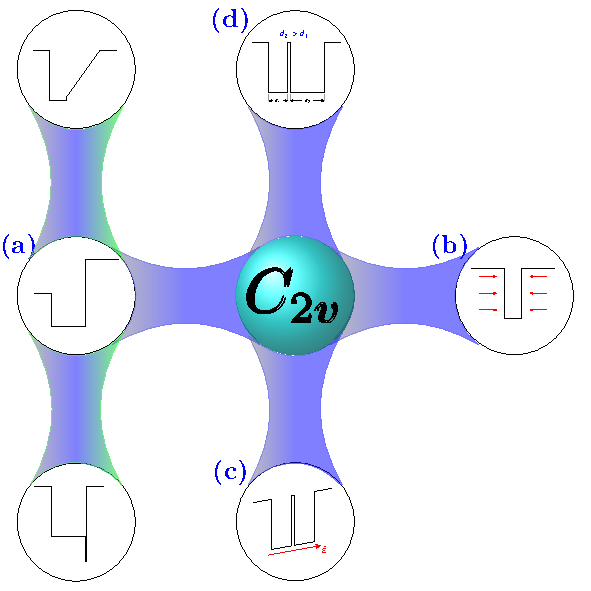
\includegraphics[width=\textwidth]{../figures/chapter-2/symmetry/out/roadmap}
		\phantomsubcaption\label{subfig:subsubsec:chapter-2-roadmap-a}
		\phantomsubcaption\label{subfig:subsubsec:chapter-2-roadmap-b}
		\phantomsubcaption\label{subfig:subsubsec:chapter-2-roadmap-c}
		\phantomsubcaption\label{subfig:subsubsec:chapter-2-roadmap-d}
		\phantomsubcaption\label{subfig:subsubsec:chapter-2-roadmap-e}
		\phantomsubcaption\label{subfig:subsubsec:chapter-2-roadmap-f}
	\end{subfigure}
	\caption
	{
		This roadmap it's developed around of QWs with remarkable potential profile, this mean posses a desire $C_{2v}$ symmetry. It starts with asymmetric QW \subref{subfig:subsubsec:chapter-2-roadmap-a}\cite{koopmans1998microscopic,andrada1997spin} specifically in potential, this is  due to the semiconductor difference in adjacent barriers to well. At center left \subref{subfig:subsubsec:chapter-2-roadmap-b} and bottom left\subref{subfig:subsubsec:chapter-2-roadmap-c} are asymmetric QWs, in the first case the asymmetry\cite{english2013effect,eldridge2011spinorbit} it's caused by gradied concentration in a barrier and bottom while the other case the asymmetry it's originated by insert an atom specie different of the barrier\cite{yu2015tuning}. At top center \subref{subfig:subsubsec:chapter-2-roadmap-d}, it's show the QW under strain\cite{english2011strain,tang2009well-width,li2019quantitative} which causes the reducing symmetry, while at bottom center\subref{subfig:subsubsec:chapter-2-roadmap-e} it shows the CQWs under applying electric field\cite{kwok1992giant}, the relation of both, it's the external perturbation which causes the breaking symmetry.  Finally, at right \subref{subfig:subsubsec:chapter-2-roadmap-f} it's presented the ACQWs which has a symmetry breaking due to the relative width of QWs\cite{ruiz2021optical}.  
	}
	\label{fig:subsubsec:chapter-2-special-symmetry--roadmap}
\end{figure}


Continued with the map, they have the perturbed structures, they are called like that due to they are under an external perturbation, at center top \Cref{subfig:subsubsec:chapter-2-roadmap-d} it's outlined a QW structure under strain applied, while at bottom center \Cref{subfig:subsubsec:chapter-2-roadmap-e} it's showing a QW structure under electric field applied. So that, in both exists, an external perturbation which causes a losses symmetry. Finally, it displays the ACQWs structure\Cref{subfig:subsubsec:chapter-2-roadmap-f}, in comparison with all above. It's notably that this structures  has two wells which are coupled by a thin barrier, by this reason as called Coupled Quantum Wells. Then, which is the reason by these structures are novels?.   

To discuss this answer, it's important to mention the relevance of CQWs being that  these structures are recurrent studied to observe quantum phenomena as exciton  (\gls{x}) condensation\cite{butov1994condensation,butov2002towards,grosso2009excitonic}. It's to be expected that in CQWs can measure indirect transitions, this means that in comparison with a single QWs whereby exists direct transitions  (band to band) hardly can measure these. But, the reality of the importance of CQWs being that excitons are very interested to apply in semiconductor devices, the properties of excitons and their interactions really exhibit quantum attractive properties. So,  unlike with single QW in CQWs the life of excitons increases\cite{hammack2009kinetics,golub1990longlived}, in fact, this is one of the principal reasons which that are attractive structures\cite{butov1994condensation,sivalertporn2012direct,winbow2011electrostatic}. Also, in terms of spin properties, the CQWs exhibit great potential\cite{bravo2022photoluminiscence}. Therefore, it being can discuss several interesting quantum properties in comparison that single structures. But, in comparison between CQWs, the symmetric structures need it perturbed to them exhibit these properties, while asymmetric structures are an excellent platform to study quantum properties such as holes mixing, spin, etc.  
It's then \emph{ACQWs an interesting structure which part from being artificial, to get natural perturbation\footnote{Thanks Dr. Raul for magnificent description.}}, even though, as can see doesn't are the unique structures with ``natural perturbation'' which generates a symmetry breaking, all above mentioned it's reduced to confinement way. This, is the reason to call special symmetry reduction in a structure hardly studied in several sub-areas of solid state. 


\section{Numerical Calculations}
\label{sec:chapter-2-numerical-calculations}
\vspace{-10mm} 
All the above cool properties mentioned, could not have been predicted or observed without their knowing their electronic properties. This is many times mentioned, is the fingerprint of semiconductors, so, also mentioned the problem to calculate it. Here was implemented a \emph{simple} model-based in \gls{efa} method to calculate the confined energies in \gls{CQWs} structures. Before explaining the numerical method to obtain these solutions, it is important to discuss the reason which can apply this method, so, it starts with the definition of band-edge from energy dispersion. In \Cref{subsec:chapter-1-valence-and-conduction-bands} are discussed in general the oncept of \gls{VB} and \gls{CB}, also is mentioned the significant methods to calculate them, in case of a heterostructure as \gls{CQWs} the complexity is greater than bulk case. In bulk, the case is well-known several methods to calculate bandstructure, where all of them are developed by the symmetry properties of the system at stake. In the case of the heterostructure, the symmetry is also important, the problem is developed a Hamiltonian capable to describe all of the system, this means, building a Hamiltonian which considers all properties as symmetry, perturbations, and in this case the potential. This work is very hard, even though exists general Hamiltonians to heterostructures, these don't warranty the correct solutions. The history and development of methods and techniques to calculate electronic properties is an area in constant evolution, from the fifties with Kane\cite{kane1957bandstructure}, Luttinger and Kohn\cite{Luttinger1955motion} in perturbed methods as \gls{kp} to Slater and Koster\cite{slater1954simplified} which proposed an atomistic method based on a linear combination of atomic orbitals called as \gls{TB}, all of this already discussed and mentioned. So, we developed a model to calculate the confined energies in coupled structures. Even though exist analytical methods to calculate confined energies, in case of CQWs is more difficult to get an exact analytical method, while also exist some analytical methods under approximation description\cite{yariv1985approximate,fromherz1997floquet,rosencher2002optoelectronics}. In the \Cref{subsection:chapter-1-preliminary-approach-of-quantum-confinment-effect-in-qws} it's developed the analytical solution of a simple quantum well taken into account the \gls{efa} method. It's possible to use this type of methods due to the symmetry reduction from bulk to QW, this due to the split in \gls{VB} which passes from being a fourfold degenerate to be a twofold degenerate. It's precisely in \gls{VB} where is it complicated to solved it. 


\begin{figure}[h!]
	\centering
	\begin{subfigure}{\textwidth}
		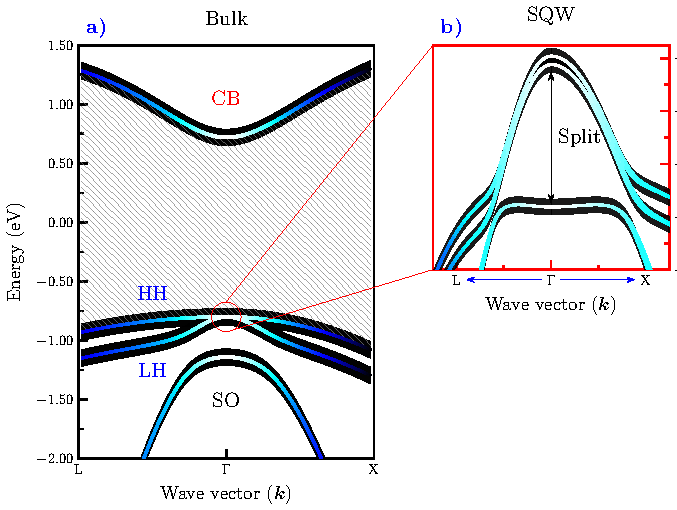
\includegraphics[width=\linewidth]{../figures/chapter-2/numerical-calculations/out/kp-bands}
		\phantomsubcaption\label{subfig:chapter-2-sec-numerical-calculations-kp-bands-bulk-a}
		\phantomsubcaption\label{subfig:chapter-2-sec-numerical-calculations-kp-bands-sqw-b}
	\end{subfigure}
	\caption[\subref{subfig:chapter-2-sec-numerical-calculations-kp-bands-bulk-a} The GaAs band structure calculated with 8-band Khane Hamiltonian\cite{kane1957bandstructure,novik2005bandstructure}]
	{
	\subref{subfig:chapter-2-sec-numerical-calculations-kp-bands-bulk-a} The GaAs band structure calculated with 8-band Khane Hamiltonian\cite{kane1957bandstructure,novik2005bandstructure}, therefore SOC is consider. At $\Gamma = 0$ in Bulk VB is closed by a circle, here observed the degeneracy, while in \subref{subfig:chapter-2-sec-numerical-calculations-kp-bands-sqw-b} it's denoted the split ($\Delta$) between heavy- and light hole bands. Also due SOC consideration, it displays the spin up and down, bands. 
	}\label{fig:chapter-2-sec-numerical-calculations-kp-bands}
\end{figure}


The \Cref{fig:chapter-2-sec-numerical-calculations-kp-bands} it's the result of apply \gls{kp} method, specifically taken into account 8-band model Hamiltonian\cite{kane1957bandstructure,galeriu2005k,vurgaftman2020bands} which is an extension of four band model\cite{galeriu2005k} and even, this model is raised to bulk semiconductors, but in \Cref{subfig:chapter-2-sec-numerical-calculations-kp-bands-sqw-b} shows the results applied in a GaAs SQW heterostructure. To give support to these calculations is important to invoke \gls{ema}, this method is an efficient method to computational calculations\cite{yeo2020first,harrison2016quantum} and their basis allows developed electron solutions. In general,  exist a variety of Hamiltonian intending to calculate the bandstructure of heterostructures. From conventional Luttinger-Kohn model, \cite{Luttinger1955motion} to relatively recent models by Burt and Foreman \cite{burt1988aneweffective,foreman1993effective,burt1992justification}, which they consider the basis functions depends on symmetry, this is the reason which  Hamiltonian is associated to the bulk structure as in this case is Zinc-Blende type. 

Although it has been discussed applying this method over heterostructures as the QWs, this work considers it as an ``exploratory'' tool. The reason for taking him into account in that way is basically their difficult and tedious way to get a correct Hamiltonian that describes our structures, in fact, \gls{kp} isn't the unique difficult method, also \gls{tb} and others, have laboriousness way to build their Hamiltonians. So, we take the technic and equations from Vurgaftman \cite{vurgaftman2020bands} and solve it numerically to gets the GaAs bulk as shown in \Cref{subfig:chapter-2-sec-numerical-calculations-kp-bands-bulk-a} and in the same route, we take the Hamiltonian from Marchewka\cite{marchewka2017finite,novik2005bandstructure} and solve under \gls{FDM}, without major preamble the idea is to denote the split between heavy- and light-hole bands which is the justification to our numerical calculations proposed. In \Cref{eqn:chapter-2:section-numerical-calculations-8x8-hamiltonian} it's presents the $8\times 8$ Hamiltonian solved to get bandstrcuture to GaAs SQW.

\begin{equation}\label{eqn:chapter-2:section-numerical-calculations-8x8-hamiltonian}
  H_{0}={\footnotesize\begin{bmatrix}
T & 0  &-\dfrac{1}{\sqrt{2}}Pk_{+}& \sqrt{\dfrac{2}{3}} Pk_{z}   & \dfrac{1}{\sqrt{6}}Pk_{-} & 0 & \dfrac{-1}{\sqrt{3}}Pk_{z} & -\dfrac{1}{\sqrt{3}}Pk_{-}\\

0 & T & 0& -\dfrac{1}{\sqrt{6}}Pk_{+}& \sqrt{\dfrac{2}{3}} Pk_{z}& \dfrac{1}{\sqrt{2}}Pk_{-}  &-\dfrac{1}{\sqrt{3}}Pk_{+}& \dfrac{1}{\sqrt{3}}Pk_{z}\\

-\dfrac{1}{\sqrt{2}}k_{-}P & 0 & U+V & -\bar{S}_{-} & R & 0 & \dfrac{1}{\sqrt{2}}\bar{S}_{-} & -\sqrt{2}R\\

\sqrt{\dfrac{2}{3}} k_{z}P&-\dfrac{1}{\sqrt{6}}k_{-}P& -\bar{S}^{\dagger}_{-}&U-V&C&R&\sqrt{2}V&-\sqrt{\dfrac{3}{2}}\tilde{S}_{-}\\
\dfrac{1}{\sqrt{6}}k_{+}P & \sqrt{\dfrac{2}{3}}k_{z}P&R^{\dagger}&C^{\dagger}&U-V&\bar{S}^{\dagger}_{+}&-\sqrt{\dfrac{3}{2}}\bar{S}_{+}&-\sqrt{2}V\\
0&\dfrac{1}{\sqrt{2}}k_{+}P&0&R^{\dagger}&\bar{S}_{+}&U+V&\sqrt{2}R^{\dagger}&\dfrac{1}{\sqrt{2}}\bar{S}_{+}\\
-\dfrac{1}{\sqrt{3}}k_{z}P&-\dfrac{1}{\sqrt{3}}k_{-}P&\dfrac{1}{\sqrt{2}}\bar{S}^{\dagger_{-}}&\sqrt{2}V&-\sqrt{\dfrac{3}{2}}\bar{S}^{\dagger}_{+}&\sqrt{2}R&U-\Delta&C\\
-\dfrac{1}{\sqrt{3}}k_{+}P&\dfrac{1}{\sqrt{3}}k_{z}P&-\sqrt{2}R^{\dagger}&-\sqrt{\dfrac{3}{2}}\bar{S}^{\dagger}_{-}&-\sqrt{2}V&\dfrac{1}{\sqrt{2}}\bar{S}^{\dagger}_{+}&C^{\dagger}&U-\Delta\\
\end{bmatrix}}
\end{equation}
where 
\begin{align*}
	k^{2}_{\parallel}&=k_{x}^{2}+k^{2}_{y},  k_{\pm}=k_{x}\pm ik_{y},  k_{z}=i\partial/\partial z,\\
	T&=E_{c}(z)+\dfrac{\hbar^{2}}{2m_{0}}\left[(2F+1)k^{2}_{\parallel}+k_{z}(2F+1)k_{z}\right], \\
	U&=E_{v}(z)-\dfrac{\hbar^{2}}{2m_{0}}\left(\gamma_{1}k^{2}_{\parallel}+k_{z}\gamma_{1}k_{z} \right),\\ 
	V&=-\dfrac{\hbar^{2}}{2m_{0}}\left(\gamma_{2}k^{2}_{\parallel}-2k_{z}\gamma_{2}k_{z}\right),\\ 
	R&=-\dfrac{\hbar^{2}}{2m_{0}}\sqrt{3}\left(\mu k^{2}_{+}-\bar{\gamma}k^{2}_{-},\right),\\
	\bar{S}_{\pm}&=-\dfrac{\hbar^{2}}{2m_{0}}\sqrt{3}k_{\pm}\left(\left\lbrace\gamma_{3},k_{z}\right\rbrace+\left[\kappa,k_{z}\right]\right),\\
	\tilde{S}_{\pm}&=-\dfrac{\hbar^{2}}{2m_{0}}\sqrt{3}k_{\pm}\left(\left\lbrace\gamma_{3},k_{z}\right\rbrace,\dfrac{1}{3}\left[\kappa,k_{z}\right]\right),\\
	C&=\dfrac{\hbar^{2}}{2m_{0}}k_{-}\left[\kappa,k_{z}\right]
\end{align*}

and each of these parameters taken from \cite{vurgaftman2020bands}. The Hamiltonian $H_{0}$ is defined for $\left[001\right]$, and the principal idea is evaluating it in a ``discrete'' SQW structure, the ''discrete`` term refers to a numerical technique for solving it. The results it shows in \cref{subfig:chapter-2-sec-numerical-calculations-kp-bands-sqw-b}, this approximation is enough to evince the \gls{VB} split, even, the results also \gls{CB} information the importance falls on  \gls{VB}, this is due that difficult to solve there.  Then, the VB split allows applying ``simple'' numerical methods without needing to define complex Hamiltonian and many parameters. In next section it will discuss the physical and mathematical formulation to calculate the electron energy confined, beginning with the symmetry reduce causes the \gls{VB} split and developed all around of $\Gamma =0$ this means we work over band-edge potential in real space. 


\subsection{Envelope Function and Effective Mass Aproximation Methods}
\label{subsec:chapter-2-efa-and-ema}
\vspace{-10mm} 
Furthermore, to get a numerical method and solution robustness without any complex formalism but based on the essence of this work which is the effect of asymmetric width potential in CQWs which causes the symmetry breaking and this physical property involve important optical phenomena, as increase Anisotropy depending on relative width in these.
The \gls{efa} is the mathematical justification to model electron behavior under periodic potential as a crystal, while the \gls{ema} is the physical model and the considerations to study the electron behavior inside a periodic potential from a crystal\cite{harrison2016quantum}\footnotetext{Frequently the \gls{efa} and \gls{ema} approximations are considered as the same term,  although maybe being correct, given that one depends on the another, is important to remark that the \gls{ema} depends on the formalism of \gls{efa}.}.
Under that assumptions, it's possible to review several considerations, that considerations reduce the complexity of solutions and allow simplifying the calculations. Then, in all of this work  it develops around of  $\Gamma=0$, this means that will use a one-band model. To resume this last context, it's importantly to taken into account the next considerations. Firstly, from here we can study the electron and holes behavior by separately, from basic assumption which $\Gamma=0$ this enables to pass from electronic band to band edge (see \Cref{fig:chapter-2-sec-numerical-calculations-band-edge}). So, it's important to define that tools previosuly mentioned. The \gls{ema} is a valid approximation in bulk materials, in fact this is an elemental model which  due to the good results and simplicity it's can be applied over heterostructures.  About of this last, the heterostructures are complex, the dissimilar matched semiconductors which conformed that it, posses doesn't only difference in band-gap energy but also the effective mass.  

\begin{figure}
	\centering
	\begin{subfigure}{\textwidth}
	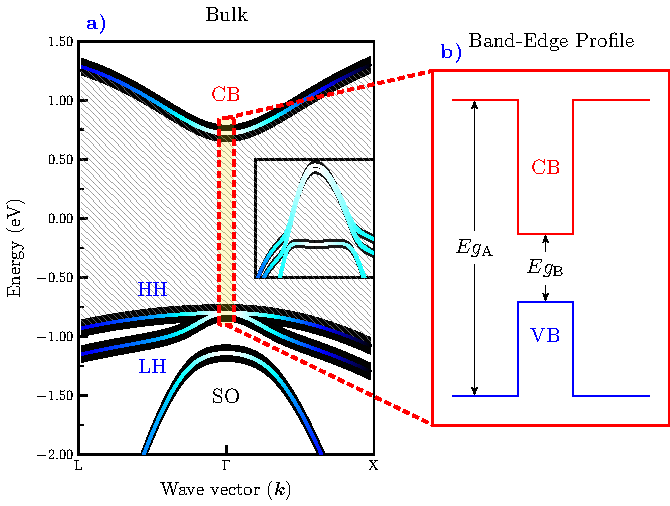
\includegraphics[width=\textwidth]{../figures/chapter-2/numerical-calculations/out/band-edge}
	\phantomsubcaption\label{subfig:chapter-2-sec-numerical-calculations-band-edge-a}
	\phantomsubcaption\label{subfig:chapter-2-sec-numerical-calculations-band-edge-b}
	\end{subfigure}
	\caption{\subref{subfig:chapter-2-sec-numerical-calculations-band-edge-a} it's tyhe focus over $\Gamma=0$ and inside is the SQW VB $\boldsymbol{k}\bigcdot \boldsymbol{p}$ results,  while the  }
	\label{fig:chapter-2-sec-numerical-calculations-band-edge}
\end{figure}

If join all of that parameters involved it, the model to solve should being proportional to the considers in it, by this reason models as \gls{TB} are complex due to the difficult to define all that parameters, while in \gls{kp} are well-defined, but contrary, the method frequently is  submitted to discussion due to the assumptions as the doesn't ``see'' the correct point-group symmetries, in fact, frequently assumes which the system already owns it.  We can introduce ourselves in a severe discussion about of bandstructure calculations methods, but the reality is can't define a standard method, so that, doing reference to Harrison et al.\cite{harrison2016quantum}, we can apply the simplicity method.
Then, assuming the simplicity term, in which practically mentioned that, it's important to consider the simple way to get a result as a long as this works. So, in this work, will discuss the increase of the  \gls{oa}  due to the relative width in the wells of the coupled system, then here only considers the potential profile as a really significant parameter, of course, the effective mass and   the band-gap are also essential, but these are considers as a part of the model. Being this the basis of the model, this work will employ the formalism of \gls{efa} where in a general explain, this it  gives the envelope functions to calculate the single electron behavior under periodic potential as a heterostructure, therefore, this can allow describing it  through position-depend material properties\cite{foreman1996envelope,benduke1966spacecharge,bastard1990wave}, then it's also indispensable to declare the boundary conditions owned by the \gls{efa}. Therefore with a mathematical formalism, then it's employed the \gls{ema} which parts of the fundamental  parameter which is the effective-mass, then it can works with the 1D-\sch's equation as a function of effective-mass, as traditional egen-value equation:

\begin{equation}\label{eqn:chapter-2-sec-numerical-calculations-eigen-value-equation}
	\textbf{H}\psi(z)=E\psi(z)
\end{equation}

Then, the Hamiltonian of \gls{ema} it's developed mainly by the effective-mass, this has the advantage of evaluated along of heterostructure,  allowing  the change of semiconductors which composed that, so, this makes it a great method. Therefore the Hamiltonian for a particle is given by\cite{kamizato1989excitons,bastard1990wave,foreman1996envelope}:

\begin{equation}\label{eqn:chapter-2-sec-numerical-calculations-ema-hamiltonian}
	H_{z} = \dfrac{p_{z}^{2}}{2m^{*}(z)}+V(z).
\end{equation}


In \Cref{eqn:chapter-2-sec-numerical-calculations-ema-hamiltonian} it's taken $z$-axis as a direction perpendicular to interface of QWs, or simply as the growth direction, consequently the potential $V(z)$ it's depend on, and the effective-mass $m^{*}(z)$ also depends on position $z$. The \Cref{eqn:chapter-2-sec-numerical-calculations-ema-hamiltonian} it's taken $z$-axis as a direction perpendicular to interface of QWs, or simply as the growth direction, consequently the potential $V(z)$ it's depend on, and the effective-mass $m^{*}(z)$ also depends on position $z$. As can see in \Cref{subfig:chapter-2-sec-numerical-calculations-band-edge-b}, it's showing the band-edge profile as a potential profile which depends on semiconductor band-gap along of heterostructure.  Also in \Cref{eqn:chapter-2-sec-numerical-calculations-ema-hamiltonian}, it considers the momentum as $p_{z}^{2}$ as a \gls{1d}, due to the before discussed. Then it's allow to developed a method to solution which depends of position $z$. Finally, it can denote a \gls{1d} \sch quation under \gls{ema} to electron also heavy- and light-holes : 

\begin{equation}\label{eqn:chapter-2-sec-numerical-calculations-ema-schrodinger}
	\begin{split}
	\left[-\dfrac{\hbar^2}{2m_{jz}^{*}}\dfrac{d^2}{dz^2}+V(z) \right]\psi_{nj}(z)&= E_{nj}\psi_{nj}(z),\\
	                                                               j&=e,\hh,\lh.
	\end{split}
\end{equation}

The \Cref{eqn:chapter-2-sec-numerical-calculations-ema-schrodinger} it's then the effective-mass equation implemented in this work. The solution of that, it's detailed in next section where explains the numerical method to solve it. Before to continue, it's important to discuss the \gls{1d} equation. This equation will be applied over each particle ($j=e,\hh,\lh$), this means, over electron, heavy- and light-holes, where only considers the effective-mass ($m_{jz}^{*}$) trough each semiconductor in heterostructure studied and the most important in this work, the potential profile $V(z)$ which depends on relative widths of coupled wells. 


\subsection{Finite Difference Method}
\label{subsec:chapter-2-finite-difference-method}
\vspace{-10mm} 
In this section it will discuss the numerical method to solve the \gls{1d} \sch's equation, even tough this is a large discussed theme, here focus on a simple but powerful numerical method. Started from the fact that the \Cref{eqn:chapter-2-sec-numerical-calculations-ema-schrodinger} can it solve along of heterostructure and taken into account each semiconductor with compose it, this means that can discretize that and solved it for electron and holes. Although this, being a \gls{1d} equation, doesn't remove importance in the solution, that is to say, it's needing a robust method. It's important to remark which the spacial discretization depends on $\delta z$.
\begin{figure}[H]
	\centering
	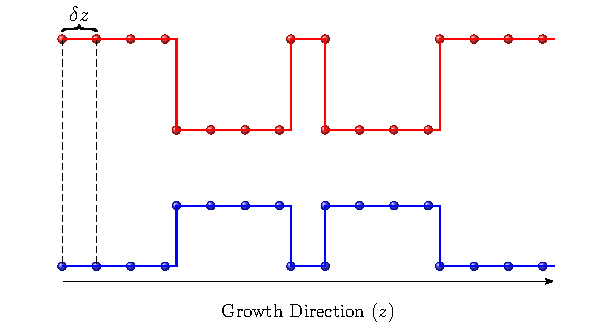
\includegraphics[width=\textwidth]{../figures/chapter-2/numerical-calculations/out/fdm-potential-1}
	\caption{Sketch of discrete potential band-edge profile which depends on spacial desplacement $\delta z$. HJ denotes the Heterojuntion boundary.}
	\label{fig:chapter-2-sec-numerical-calculations-fdm-potential}
\end{figure}
In \Cref{fig:chapter-2-sec-numerical-calculations-fdm-potential} schemes the discrete potential profile considers, this band-edge profile corresponds to a \gls{SCQWs} structure. Remember that the potential $V(z)$ comes from the bend-edge Energy $E_{edge}$, like in the \gls{CB} and \gls{VB}, from that take the effective mass which corresponds to each semiconductor which compounds all heterostructure. Then, we can divide a heterostructure with coupled quantum wells basically into two parts, the adjacent barriers and the zone of wells which is considered the coupled barrier and their width as well as the relative widths of each well. So, if consider the discrete structure we can apply \Cref{eqn:chapter-2-sec-numerical-calculations-ema-schrodinger} in each point which composes that. 

The solution of \Cref{eqn:chapter-2-sec-numerical-calculations-ema-schrodinger} it's the central discussion, although exist several numerical methods to solve it, in this work is employed the \emph{Finite Difference Method} (\gls{FDM}), which begin characterized by the easy computational application. Even if, this method doesn't unique in applied discretization in comparison with the other method as Shoting\cite{killingbeck2020microcomputer,harrison2016quantum}, reduce the computational time and assure the correct convergence as long as the boundary conditions are correct. In other words, the \gls{FDM} is a non-sensible convergence method, being focused on matrix solution.  Taking the \Cref{eqn:chapter-2-sec-numerical-calculations-ema-schrodinger} and reformulated as a \emph{difference equation}\cite{harrison2016quantum}:
\begin{equation}\label{eqn:chapter-2-sec-numerical-calculations-schrodinger-discrete}
	-\dfrac{\hbar}{2m^{*}}\left[\dfrac{\psi(z+\delta z)-2\psi(z)+\psi(z-\delta z)}{(\delta z)^2}\right] + V(z)\psi(z)=E\psi(z).
\end{equation}

In the \Cref{eqn:chapter-2-sec-numerical-calculations-schrodinger-discrete} it's denoted the derivative change by numerical difference,  being a discrete equation. Something that it's important to consider is the boundary conditions which depend on the number of semiconductors involves in the structure and their dimensions, then, if it requires high precision it's important two factors: the total dimension of the structure, which contemplates each heterojunction boundary and the spatial step defined by $\delta z$. Either way, if considering a wide structure, as well as a very small step ($\delta z \approx 1\AA$) the computational effort, is high, for this reason, the compute considered memory should be reasonable.Then, taking into account these two factors and considering the computational work, the best choose a Matrix solution.

The Matricial solution allows solving the system of equations naturally as an eigenvalue problem, then it has several numerical alternatives\footnote{This refers to linear algebra techniques\cite{harrison2016quantum,davidson1993monster}} to solve the system. The reason to assert these has to do with the discrete solution as large as the ratio between structure width and spatial step. This means the matrix has  dimensions as : $N = \text{total width}/\delta z$. Then, the way to get matrix ($\textbf{H}$), from Harrison et al. \cite{harrison2016quantum}, consists in reformulate  \Cref{eqn:chapter-2-sec-numerical-calculations-schrodinger-discrete} as function of spatial potential band edge taken into account the variable effective mass, then:

\begin{equation}\label{eqn:chapter-2-sec-numerical-calculations-schrodinger-discrete-to-matrix}
	a_{i}\psi_{i-1}+b_{i}\psi_{i}+c_{i}\psi_{i+1}=E\psi_{i}
\end{equation}
where the coefficients are:

\begin{equation}\label{eqn:chapter-2-sec-numerical-calculations-schrodinger-discrete-to-matrix-coefficients}
	a_{i+1}=c_{i}= -\dfrac{\hbar^2}{2m^{*}_{i+\frac{1}{2}}(\delta z)^2} \quad \text{and}\quad b_{i}=\dfrac{\hbar^{2}}{2(\delta z)^2}\left(\dfrac{1}{m^{*}_{i+\frac{1}{2}}}+\dfrac{1}{m^{*}_{i-\frac{1}{2}}}\right)+V_{i}
\end{equation}

From \Cref{eqn:chapter-2-sec-numerical-calculations-eigen-value-equation}, then the matrix \textbf{H} is conformed by the system of equations which is evaluated in each point os structure, then \textbf{H} is:  
\begin{equation}
	\textbf{H}=\begin{pmatrix}
		b_{1} & c_{1} & 0      &\cdots & 0\\
		a_{2} & b_{2} & c_{2}  &\cdots &0\\
		0     &\ddots &\ddots  &\ddots&0\\
		\vdots&\cdots &a_{N-1} &b_{N-1}&c_{N-1}\\
		0     &\cdots&0        &a_{N}  &b_{N} 
	\end{pmatrix}
\end{equation}
then $\psi$ is in \Cref{eqn:chapter-2-sec-numerical-calculations-eigen-value-equation} is a vector column which containing all the samples of the wave function. 

Then, for the solution of the $N\times N$ matrix it's represents a computation work, but due to the \emph{tridiagonal} nature it reduces that effort and thanks to exist great algebraic algorithms to solve\cite{laug1999lapack,harris2020array}, this work can simplify enormous. 
Therefore, this method simplifies the solution of any structure with arbitrary or in our case dependent on band-edge potential. The next task is over to define the potential profile and their dependence of  effective-mass and band gap energy (\gls{eg}).  Firstly, we take as reference the double quantum wells propose by Harrison et al.\cite{harrison2016chap3} and reproduce the  eigenenergies and wave functions as shows in \Cref{fig:chapter-2-sec-numerical-calculations-harrison-wells}.For this structure, it takes into account symmetric double wells, that is to say, with same width $l_{w}=6$nm, \algaasx{0.2} central barrier of $l_{b}=4$.  For the semiconductor parameters with compose that structure, as the model like shows in the \Cref{eqn:chapter-2-sec-numerical-calculations-ema-schrodinger} doesn't take into account the effective mass as energy function and not taken into account the nonparabolicity\cite{nelson1987band,cooper2010finite}. Then, to define potential profile $V(z)$ uses the Varshni's model \cite{varshni1967temperature}, to calculate bandgap energy to GaAs/\algaas, how doesn't consider the mass-effective as energy dependence then it uses paramaters from: \cite{vurgaftman2001bandparameters,molenk1988determination,adachi2009properties,lew2009heterostructuresbasicformalism}, finally it employs the Vegard's law to define the thernary semiconductors\cite{donmez2012study,zhou2001deviation}. If defines the potential profile as:
\begin{equation}\label{eqn:chapter-2-sec-numerical-calculations-harrison-potential-profile}
	V(z),m^{*}(z)=\begin{cases}
		\text{\algaasx{0.2}}\quad &0<z<20\text{ nm}\\
		\text{GaAs}\quad    &20<z<26\text{ nm}\\
		\text{\algaasx{0.2}}\quad &26<z<32\text{ nm}\\
		\text{GaAs}\quad    &32<z<38\text{ nm}\\
		\text{\algaasx{0.2}}\quad &38<z<58\text{ nm}
	\end{cases}
\end{equation}

\begin{figure}[H]
	\centering
	\begin{subfigure}{\textwidth}
	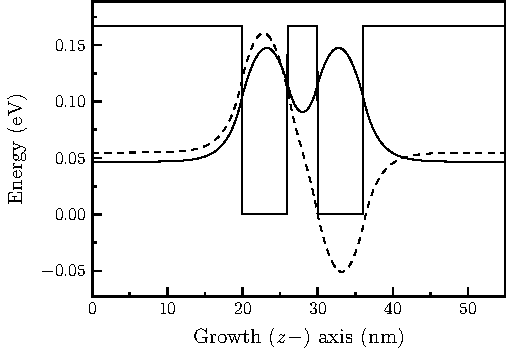
\includegraphics[width=\textwidth]{../figures/chapter-2/numerical-calculations/out/harrison-wells}
	\phantomsubcaption\label{subfig:chapter-2-sec-numerical-comparison-harrison-plot-a}
	\phantomsubcaption\label{subfig:chapter-2-sec-numerical-comparison-harrison-table-b}
	\end{subfigure}
	\caption{Doble Quantum Wells structure reproduce from  Harrison et al.\cite{harrison2016chap3}, \subref{subfig:chapter-2-sec-numerical-comparison-harrison-plot-a} shows the plot to each energy calculate $e_{1}$ and $e_{2}$, while in \subref{subfig:chapter-2-sec-numerical-comparison-harrison-table-b} the table exposes the comparison of  numerical results from \textbf{Harrison} et. al., \textbf{Nextnano} software \cite{Nextnanoharrison} and our results. The difference taken into account the Harrison's results practically are the same, but around of meV orders our results are precisely.  }
	\label{fig:chapter-2-sec-numerical-calculations-harrison-wells}
\end{figure}
where the $V(z)$ it defines by the correspond value of \gls{eg} and the effective-mass $m^{*}(z)$, both with the spatial $z$ dependence. But, this work as only in take \textbf{Harrison} et al.\cite{harrison2016quantum} like a reference, the \textbf{Nextnano} software\cite{birner2007Nextnano,Nextnanoharrison} also take that, in the \Cref{fig:chapter-2-sec-numerical-calculations-harrison-wells} and \Cref{subfig:chapter-2-sec-numerical-comparison-harrison-table-b} shows the table of comparison results, taken as basis \textbf{Harrison} et al. and compare also with  \textbf{Nextnano} software and the codes developed in this work \cite{cqws-codes}. As can see, the results getting in this work are precise with respect to Harrison, and it's important to remark this work doesn't intend to denote supremacy since that fall short of sense, the intent is only the comparison to demonstrate that our codes works. The table in \Cref{subfig:chapter-2-sec-numerical-comparison-harrison-table-b} it denotes (with red) the precision around of meV, this is what we mean when say the major precision with respect to Harrison's results. 
Thus, we can trust the codes and model here present, do they work concerning with computational aspect and the physical results, and although only focused over electrons' solution in the band-edge profile, the next part of this works presents the results obtained in the interest structures. 
\section{Numerical Results}
\label{sec:chapter-2-numerical-results}
\vspace{-10mm} 
Here, we introduce the results obtained in \gls{CQWs} studied in this work.\Cref{sec:chapter-3-section-samples-description} it's detailed of the structures' composition as well as the properties of these. Then, here focus only in the  numerical and computational results, over all, in the calculation of confined energies it remembers that our model is oriented only about energies, so that, frequently explain many parameters and arguments that doesn't consider here. But, that doesn't mean which the obtained results minimize the quality of this work, in fact, we achieve very interest results without need to draw on to the very hard models.The \Cref{fig:chapter-2-sec-numerical-calculations-results} shows the plot of wave functions for electrons, heavy- and light-holes resultant of numerical calculations, here taken into account only four samples detailed in \Cref{sec:chapter-3-section-samples-description} at the \Cref{tab:chapter3:Samples description}, all of these samples are the CQWs structures studied in this work, then over each of these was calculated the confined energies and the wave functions profiles. In the \Cref{fig:chapter-2-sec-numerical-calculations-results} it's calculated $\psi$ to denoted more clarify the overlapping wave functions over two coupled wells, even tough here doesn't show the total table of confinement energies results, later these will  compare with the experimental transitions.  Therefore, in this section, we limited to specify the numerical results  in accordance with the published work\cite{ruiz2021optical}. 
\begin{table}[H]
	\centering
	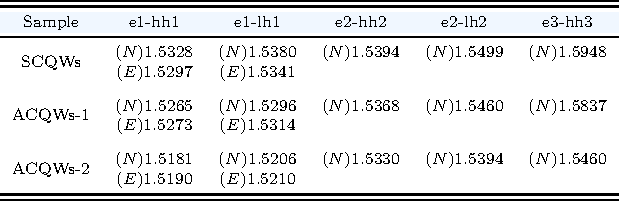
\includegraphics[width=\textwidth]{../tables/chapter-2/numerical-results/out/numerical-results.pdf}
	\caption{Direct transitions ($\mathbf{X}$) calculated for two ACQWs and one SCQW detailed in \Cref{sec:chapter-3-section-samples-description} and \Cref{tab:chapter3:Samples description}. From uo to down shows the numerical (E) and experimental results, the experimental results was obtained from RAS experiments which are performed at 30K. }
	\label{tab:sec-chapter-2-numerical-results} 
\end{table}
In the \Cref{tab:sec-chapter-2-numerical-results} exposes and compares the numerical results obtained, it's importantly to remark that the calculations were performed at 30K, this due to the central experiments (RAS) are performed to that temperature, by this reason the parameters involves are well-defined as a function of temperature. These calculations taken into account the conduction and valence-band offsets of 65\% and 35\% respectively. Both electron and hole effective masses for GaAs and AlAs can be found in Refs.\cite{vurgaftman2001bandparameters,molenk1988determination,adachi2009properties}, whereas the ternary \algaas we used the Vegard's law\cite{donmez2012study}. For the numerical direct transitions (\gls{x}) calculated, it's consider the exciton binding energy as a function of well width \cite{yutaka1994theeffect,greene1984energylevels}, as commonly  only shows the direct transitions in a range of wells widths, we interpolate these energies to  used in accordance with the structures used in  this work. 
The \Cref{fig:chapter-2-sec-numerical-calculations-results} denotes some interesting physical issues, one of these with principal role in this work it's a linked between barrier width and the relative width of the coupled wells. 
\begin{figure}[H]
	\centering
	\begin{subfigure}{\textwidth}
	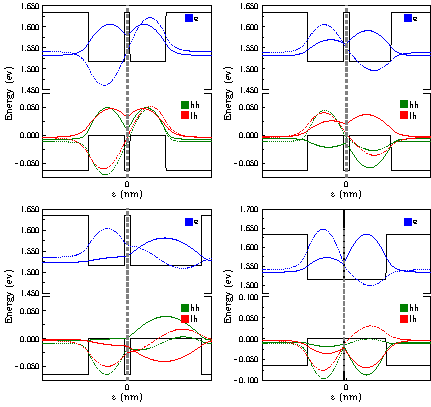
\includegraphics[width=\textwidth]{../figures/chapter-2/numerical-calculations/out/numerical-results}
	\phantomsubcaption\label{subfig:chapter-2-sec-numerical-results-a}
	\phantomsubcaption\label{subfig:chapter-2-sec-numerical-results-b}
	\phantomsubcaption\label{subfig:chapter-2-sec-numerical-results-c}
	\phantomsubcaption\label{subfig:chapter-2-sec-numerical-results-d}
	\end{subfigure}
	\caption{From \subref{subfig:chapter-2-sec-numerical-results-a} a to \subref{subfig:chapter-2-sec-numerical-results-d} shcemes the numerical results obtained to solved 1D-Schrödinger equation in both SQWs and ACQWs. }
	\label{fig:chapter-2-sec-numerical-calculations-results}
\end{figure}               
The barrier width as can see plays an important role, because the width define tunneling of electrons and holes, for example \Cref{subfig:chapter-2-sec-numerical-results-b} and \Cref{subfig:chapter-2-sec-numerical-results-d}  structures has the same wells widths with exception to barrier type, the first one is \algaasx{0.15} and the width is $b_{w}=1.98$nm while the second one is AlAs type with a width of $b_{w}=0.565$nm. It's known that the difference between these is the bandgap energy then, as is expected, the tunneling is less than the \algaasx{0.15}  barrier. Concerning tunneling, if compares the \Cref{subfig:chapter-2-sec-numerical-results-a} and \Cref{subfig:chapter-2-sec-numerical-results-c} structures, which basically are the same structures except for the width of the second well, the wave function in one of these,  are symmetrically localized as a doublets states, while the other the wave function practically is well localized in one of the wells as single state energy of a single QW\cite{sivalertporn2016effectofbarrier}. While if compares with \Cref{subfig:chapter-2-sec-numerical-results-b} where one of the coupled wells is slightly  width than the other, the wave function distribution seems an SQCWs under applied external electric field\cite{sivalertporn2012direct},later in \Cref{subsec:chapter-3-pr} this take a sense, in \gls{PR} experiments appear transitions which we associated to three-body particles known as trions (\gls{ntrion} or \gls{ptrion}). Trions are particular particles that consist of the bound of two electrons and one hole (\gls{ntrion}) or vice versa, two holes and one electron (\gls{ptrion}).The fact of one of the wells is slightly width, entails quantum interactions measured experimentally. But, this doesn't only the unique, interesting phenomena observed in these structures. As before mentioned this work, focuses on the optical properties consequent of the structural asymmetry, this means, the relative width in double wells. 
\section{Anisotropy model in CQWs \label{sub:chap2-anisotropy-model}}
\label{subsec:chapter-2-anisotropy-model}
\vspace{-10mm} 
Now, we focus on the central part either, the core of this work. The asymmetry in structure entails a very interesting quantum process in these semiconductor structures. The symmetry reduction is the basis of the model in this work, as explained before, symmetry is the cause of many quantum phenomena its exibits in solids, and the fact, that symmetry breaking in CQWs increases the optical anisotropy, which among many properties this opens the field of spin properties\cite{sivalertporn2012direct,averkiev2006spin,kotova2016optical,schonhuber2014inelastic,tronc2012spin}.


Generalizing the before discussed in the symmetry section exists several mechanisms to reduce symmetry in QWs structures, principally in the single QWs with external perturbations such as electric or magnetic field, mechanics perturbations as applied strain among others.  But, the objective is the same, reduce the symmetry in these structures from  $T_{d}$ which is the symmetry group to cubic crystals to $C_{2v}$ which in turn a  subgroup of this. As the result of the symmetry breaking,  it originates an OA which was measured through \gls{RAS} experiments results in a peculiar way, this refers to the spectral results. In our case, it compares the experimental results of \gls{RAS} experiments (later discussed) about three CQWs structures, in which the difference between these is only the width of one of the wells (as many times mentioned), the \gls{RAS} spectra increase as the relative width also,  this, come back to these structures very interesting.  Therefore, it will discuss the Anisotropy Model which includes all of the previous contained and focused on the CQWs. The \gls{oa} was borns as of the Quantum-mechanically effect of mixing between holes states, the theoretical formalism frequently is developed around effective mass but it's important to remember the difficulty of solid physics, now if it adds the physics of the interface this is so crazy. The role of interfaces is crucially in heterostructures in point of fact is the principal cause, then, having a standard model which explains it, is practically impossible. Therefore the \emph{simplicity method is ever the good choice.}
\begin{figure}[H]
	\centering
	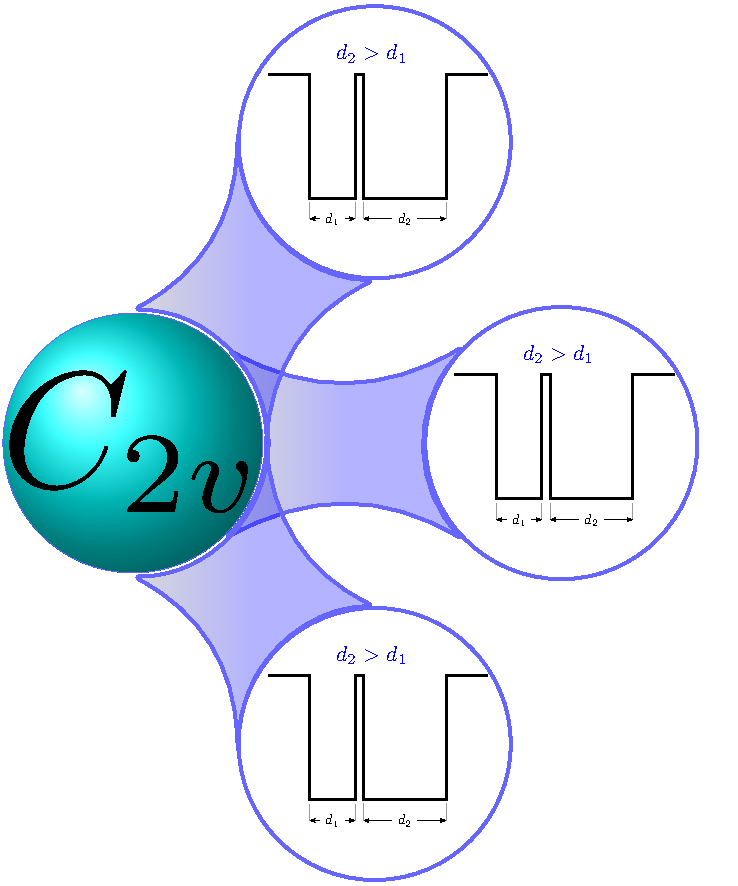
\includegraphics[width=\textwidth]{../figures/chapter-2/model/out/model-scheme}
	\caption{Diagram of three principal structures studied in this work, started with CQWs with the same width (bottom,$d_{1}=d_{2}$), this sample structure is called as SCQWs, the second one the first asymmetric structure (top, $d_{1}<d_{2}$), this means that one of the wells is slightly width than the other. Finally the third sample (right) it's more asymmetric, which means that one of the wells is double wider than the other.    }
	\label{fig:chapter-2-anisotropy-model-samples-studied}
\end{figure}
\newpage
The \gls{efa} usually employs the analytical method to explain the heavy- and light- holes states lack of interface contribution\cite{xiao2001determination}.In the fact,  always it desires high-quality interfaces but even though the growth technologies are very precise and powerful this remains a natural atom process. It's important to say that the quality of structures studied it's amazing, even in the SCQWs were expected a non-observable anisotropy due to the conserve of $D_{2d}$ symmetry, experimentally observes a remanent of anisotropy. As it's exposed in the \Cref{fig:chapter-2-anisotropy-model-samples-studied} the three  CQWs structures studied, including the symmetric double wells sample which remarks in red because this is the basis to demonstrate the evolution of anisotropy increases as the asymmetry in wells also to. 